\documentclass[11pt]{article}

\usepackage[margin=1in]{geometry}
\usepackage{amsmath,amssymb}
\usepackage{booktabs}
\usepackage[hidelinks]{hyperref}
\usepackage{tikz}
\usetikzlibrary{arrows.meta,positioning,calc}
\usepackage{graphicx}
\usepackage{float}
\usepackage{booktabs,tabularx,array}

\title{Model 1 Outline}
\author{}
\date{}

\begin{document}
\maketitle

\begin{abstract}
    This is an outline for my first model. The goal was the exercise the different components I learned about in Prince's Understanding Deep Learning. It was a successful experiement, and good practice. I have two goals the next two models will build on.
    First, I want to experiment with synthetic data, the last few chapters of the book were about generative models, so I want to try building a generative model for different bits of these two datasets. Second, I want to refine this model a bit, get some stronger results, 
    then attach a conformal predictor to it, as further practice. Since finishing Prince's book, I have begun reading "a gentle introduction to conformal prediction and distribution-free uncertainty quantification".
\end{abstract}


\section{Objective}
    The primary object is to use the pre-training plus fine-tuning paradigm, ontop of some kind of transformer 
    architecture. The most obvious choice was to do win-prediction, hence the goal is win prediction. 

    Ultimately, this sub-project is about selecting and justifying an architecture (for the given task, which may 
    not be well posed), and empirically learning about the effects of choices like optimizers, loss functions, 
    regularization techniques, and subtle architecture adjustments. All is in the service of spurring on my own 
    interest in the field.



\section{Data}
    The data for this project comes from a public Deadlock data API. It comes in two forms:
    \begin{enumerate}
        \item End-of-Match - This is essentially a screenshot of the final scoreboard. This will include variables determined by the outcome of the game, like kills, death, items, and souls, but will also have element invariant of outcome, like character selection, lane assignment, and rank (elo).
        \item Event Stream - This is literally the entire game. Every entities position at every tick of the game, every characters soul count, kills, deaths, assists, spatial position, ability cooldowns, etc. This is the ultra-high resolution spatial-temporal data that initial inspired me to consider this dataset.
    \end{enumerate}
    These two datasets provide a nice form factor for the pre-training/fine-tuning paradigm. The first, End-of-Match data, is extremely small, and easy to get, providing the usual medium for pre-training. The second, Event Stream data, provide, again, an excellent structure for this paradigm; Extremely high resolution, expensive, well labeled data. However, the event stream data also has the bonus feature that the ultra-high detail of it allows for multimodal use of the data.



\newpage 
\section{Architecture}
    The architecture I came up with is as follows:
% Final Architecture Layout
    \begin{figure}[H]
    \centering
    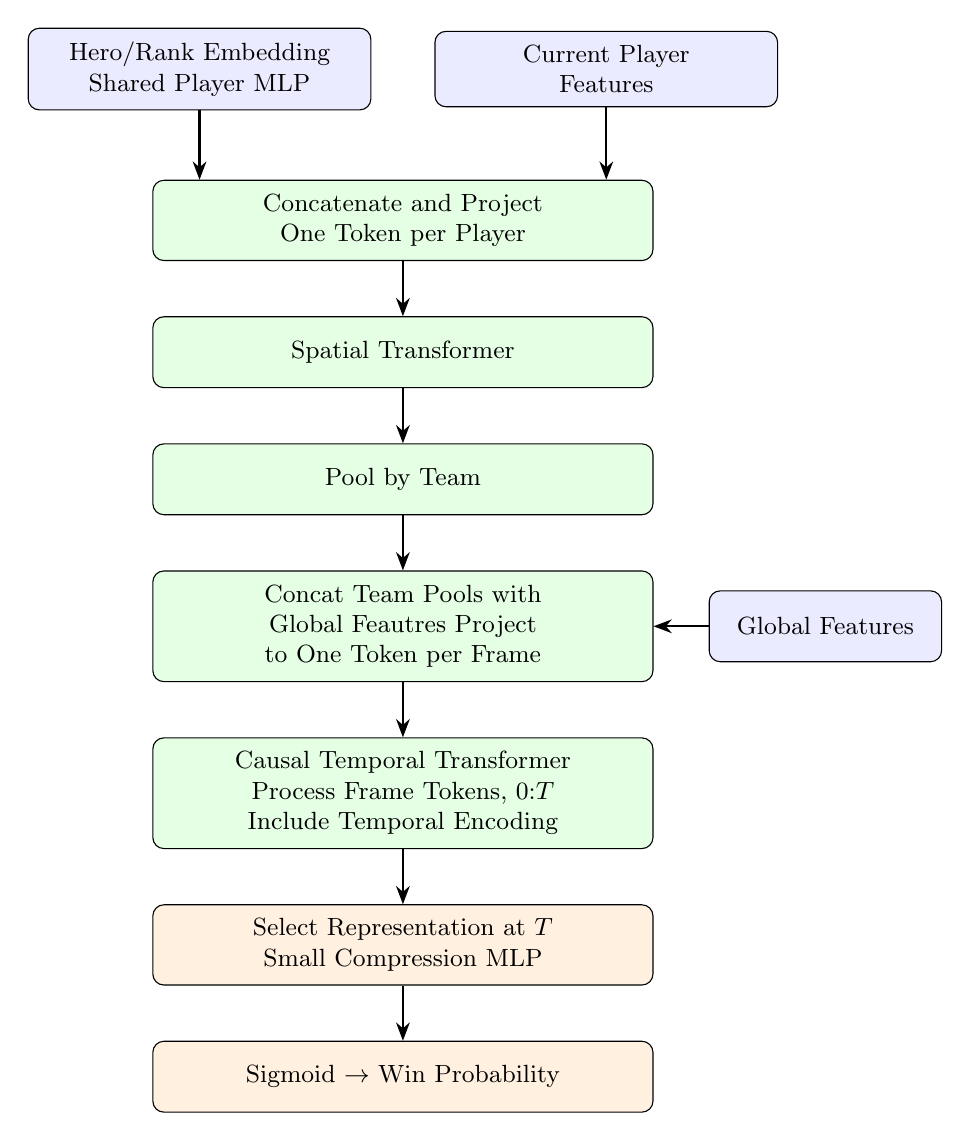
\begin{tikzpicture}[
        font=\small,
        node distance=7mm,
        box/.style={
            draw,
            rounded corners,
            align=center,
            text width=6cm,
            minimum height=9mm,
            inner sep=5pt
        },
        input/.style={box, text width=4cm, fill=blue!8},
        process/.style={box, fill=green!10},
        output/.style={box, fill=orange!12},
        arrow/.style={-{Stealth}, thick}
    ]

    \node[input] (hero) {
        Hero/Rank Embedding\\
        Shared Player MLP
    };

    \node[input, right=8mm of hero] (state) {
        Current Player\\
        Features
    };

    \coordinate (middle) at
        ($(hero.south)!0.5!(state.south)$);

    \node[process, below=9mm of middle] (concat) {
        Concatenate and Project\\
        One Token per Player
    };

    \node[process, below=of concat] (spatial) {
        Spatial Transformer
    };

    \node[process, below=of spatial] (pool) {
        Pool by Team
    };

    \node[process, below=of pool] (frame) {
        Concat Team Pools with\\
        Global Feautres
        Project to One Token per Frame
    };

    \node[input, right=7mm of frame, text width=2.6cm] (global) {
        Global Features
    };

    \node[process, below=of frame] (temporal) {
        Causal Temporal Transformer\\
        Process Frame Tokens, $0{:}T$\\
        Include Temporal Encoding
    };

    \node[output, below=of temporal] (head) {
        Select Representation at $T$\\
        Small Compression MLP
    };

    \node[output, below=of head] (win) {
        Sigmoid $\rightarrow$ Win Probability
    };

    \draw[arrow] (hero.south) --
        (concat.north -| hero.south);
    \draw[arrow] (state.south) --
        (concat.north -| state.south);
    \draw[arrow] (concat) -- (spatial);
    \draw[arrow] (spatial) -- (pool);
    \draw[arrow] (pool) -- (frame);
    \draw[arrow] (global.west) -- (frame.east);
    \draw[arrow] (frame) -- (temporal);
    \draw[arrow] (temporal) -- (head);
    \draw[arrow] (head) -- (win);

    \end{tikzpicture}
    \caption{
        Win-prediction architecture.
        Shared player encoding and spatial attention are applied
        to each frame; temporal attention combines the observed
        history to predict the final match outcome.
    }
    \label{fig:final-architecture}
    \end{figure}
\newpage
% Symbolic descriptions
    Let $\mathcal{I}$ denote the set of heroes, e.g., $\mathcal{I}=\{\text{Abrams},\text{Apollo},\text{Warden},\ldots\}$. For a given match, let $p\in\{1,\ldots,12\}$ index players and $t\in\{0,\ldots,T\}$ index observed frames. Player $p$ selects hero $i_p\in\mathcal{I}$ and has scaled pre-match rank $r_p\in\mathbb{R}_+$. Let $\mathbf{x}_{p,t}\in\mathbb{R}^{F}$ contain current player features, including team identity, position, kills and death, and let $\mathbf{g}_t\in\mathbb{R}^{G}$ contain global features like tower damage, urn count, elasped time. Let $[\mathbf{a};\mathbf{b}]$ denote vector concatenation.
% Architectural description
    \begin{table}[H]
    \centering
    \small
    \renewcommand{\arraystretch}{1.3}
    \setlength{\tabcolsep}{5pt}

    \begin{tabularx}{\textwidth}{
        >{\raggedright\arraybackslash}p{0.20\textwidth}
        >{\raggedright\arraybackslash}X
        >{\raggedright\arraybackslash}p{0.44\textwidth}
    }
    \toprule
    \textbf{Component} &
    \textbf{Purpose} &
    \textbf{Symbol \& Structure} \\
    \midrule

    Hero embedding &
    Learned hero lookup vector. &
    $e_i \in \mathbb{R}^{16}$ for each $i \in \mathcal{I}$\\

    Static player MLP &
    Condition hero representation on rank. &
    $\mathbf{s}_p=f_{\mathrm{static}}([\mathbf{e}_{i_p};r_p]) \in\mathbb{R}^{32}$ where $f_{\mathrm{static}}$ is an MLP with ReLU layers
    MLP: $17\rightarrow32\rightarrow32$\\

    Player projection &
    Combine static and current features. &
    $\mathbf{z}_{p,t} =\mathbf{W}_{\mathrm{player}} [\mathbf{s}_p;\mathbf{x}_{p,t}] +\mathbf{b}_{\mathrm{player}} \in\mathbb{R}^{64}$\\

    Spatial transformer &
    Contextualize players within a frame. &
    $\mathbf{U}_t =\operatorname{Spatial}(\mathbf{Z}_t) \in\mathbb{R}^{12\times64}$; 1 block, 4 heads, feed-forward with width 128. \\

    Team pooling &
    Summarize each team's players. &
    $\displaystyle\mathbf{a}_{k,t}=\frac{1}{6}\sum_{p\in\mathcal{P}_k}\mathbf{u}_{p,t}\in\mathbb{R}^{64}$, where $\mathcal{P}_k$ is team $k$'s player set. \\

    Frame projection &
    Combine team summaries and global state. &
    $\mathbf{v}_t=\mathbf{W}_{\mathrm{frame}}[\mathbf{a}_{1,t};\mathbf{a}_{2,t};\mathbf{g}_t]+\mathbf{b}_{\mathrm{frame}}\in\mathbb{R}^{64}$. \\

    Temporal encoding &
    Represent frame order. &
    $\tilde{\mathbf{v}}_t=\mathbf{v}_t+\mathbf{q}_t$, where $\mathbf{q}_t\in\mathbb{R}^{64}$ is a positional encoding. \\

    Temporal transformer &
    Represent observed match history. &
    $\mathbf{h}_T=\operatorname{Temporal}(\tilde{\mathbf{v}}_0,\ldots,\tilde{\mathbf{v}}_T)_T\in\mathbb{R}^{64}$; 2 blocks, 4 heads, feed-forward with width 128. \\

    Win head &
    Predict team 1's win probability. &
    $\hat{p}_T=\sigma(f_{\mathrm{win}}(\mathbf{h}_T))$; where $f_{\mathrm{win}}$ is an MLP with ReLU layers $64\rightarrow32\rightarrow1$\\

    \bottomrule
    \end{tabularx}

    \caption{
        Proposed architecture.
        $\mathbf{Z}_t$ stacks player tokens as rows;
        $\mathbf{u}_{p,t}$ is player $p$'s spatial output.
    }
    \label{tab:model-components}
    \end{table}
    Now with the architecture figured out, how to train it becomes the next major question.


\newpage
\section{Training}
    In order to meet the goals of this sub-project, and take advantage of all the available data, this is the following training procedure I have come up with for this model. Note that numerical values for parameters are initial quantities and will likely be adjusted during training.
% Graph of training order
    \begin{figure}[H]
    \centering
    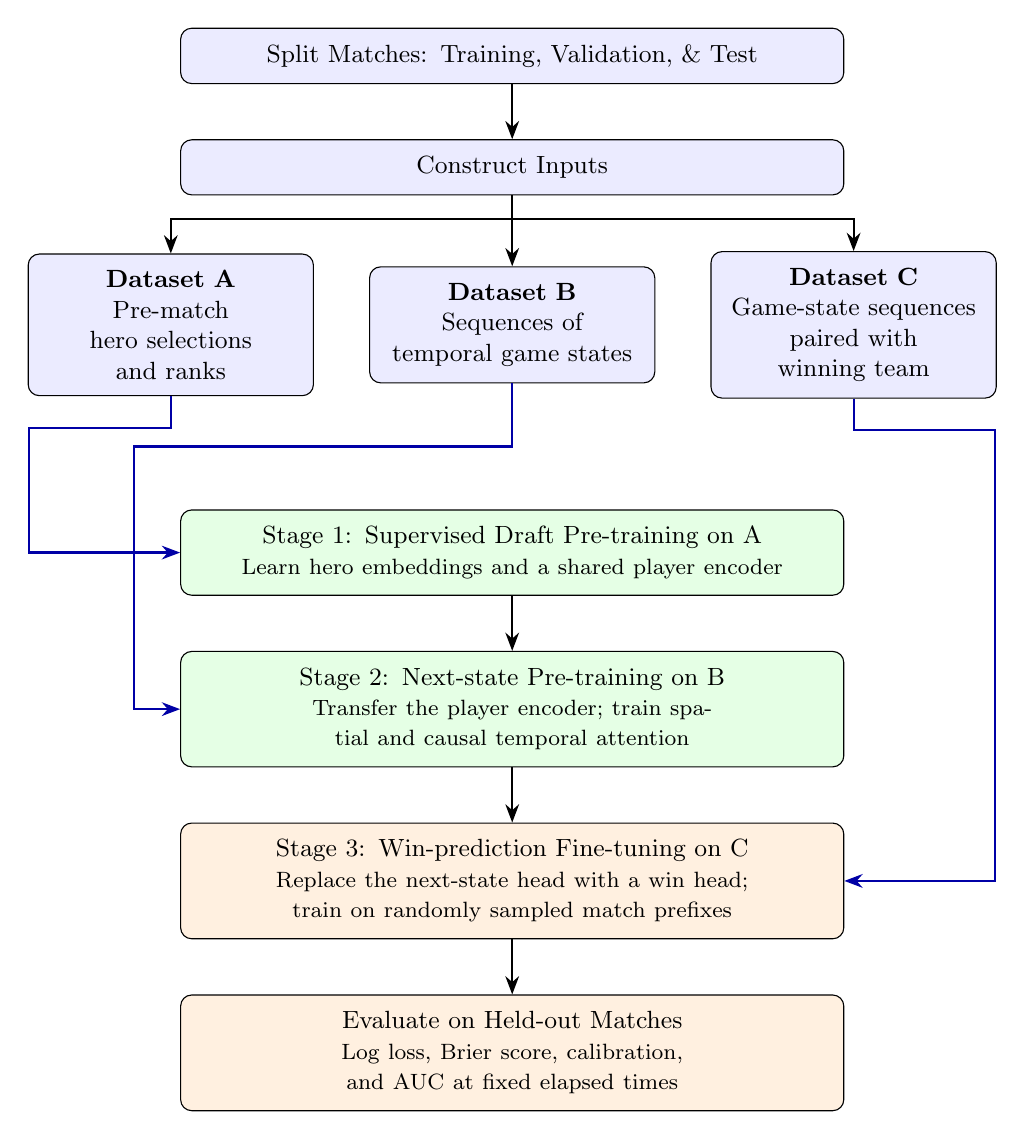
\begin{tikzpicture}[
        font=\small,
        node distance=7mm,
        box/.style={
            draw,
            rounded corners,
            align=center,
            text width=8cm,
            inner sep=6pt
        },
        data/.style={box, fill=blue!8},
        dataset/.style={data, text width=3.2cm, minimum height=1.2cm},
        train/.style={box, fill=green!10},
        final/.style={box, fill=orange!12},
        arrow/.style={-{Stealth}, thick},
        feed/.style={arrow, blue!65!black}
    ]

    \node[data] (split) {
        Split Matches: Training, Validation, \& Test
    };

    \node[data, below=of split] (inputs) {
        Construct Inputs
    };

    % Three dataset branches.
    \node[dataset, below=9mm of inputs] (B) {
        \textbf{Dataset B}\\
        Sequences of \\temporal game states
    };

    \node[dataset, left=7mm of B] (A) {
        \textbf{Dataset A}\\
        Pre-match hero selections\\
        and ranks
    };

    \node[dataset, right=7mm of B] (C) {
        \textbf{Dataset C}\\
        Game-state sequences\\
        paired with winning team
    };

    % Training stages.
    \node[train, below=16mm of B] (stage1) {
        Stage 1: Supervised Draft Pre-training on A\\
        \footnotesize
        Learn hero embeddings and a shared player encoder
    };

    \node[train, below=of stage1] (stage2) {
        Stage 2: Next-state Pre-training on B\\
        \footnotesize
        Transfer the player encoder;
        train spatial and causal temporal attention
    };

    \node[final, below=of stage2] (stage3) {
        Stage 3: Win-prediction Fine-tuning on C\\
        \footnotesize
        Replace the next-state head with a win head;
        train on randomly sampled match prefixes
    };

    \node[final, below=of stage3] (evaluate) {
        Evaluate on Held-out Matches\\
        \footnotesize
        Log loss, Brier score, calibration, and AUC
        at fixed elapsed times
    };

    % Input construction branches.
    \draw[arrow] (split) -- (inputs);
    \draw[arrow] (inputs.south) -- (B.north);
    \draw[arrow] (inputs.south) -- ++(0,-3mm) -| (A.north);
    \draw[arrow] (inputs.south) -- ++(0,-3mm) -| (C.north);

    % Dataset A enters Stage 1 from the left.
    \draw[feed] (A.south)
        -- ++(0,-4mm)
        -- ++(-1.8cm,0)
        |- (stage1.west);

    % Dataset B enters Stage 2 via a separate left-hand route.
    \draw[feed] (B.south)
        -- ++(0,-8mm)
        -- ++(-4.8cm,0)
        |- (stage2.west);

    % Dataset C enters Stage 3 from the right.
    \draw[feed] (C.south)
        -- ++(0,-4mm)
        -- ++(1.8cm,0)
        |- (stage3.east);

    % Sequential parameter transfer and evaluation.
    \draw[arrow] (stage1) -- (stage2);
    \draw[arrow] (stage2) -- (stage3);
    \draw[arrow] (stage3) -- (evaluate);

    \end{tikzpicture}
    \caption{
        Proposed training procedure.
        Blue arrows supply each stage with its corresponding dataset;
        black arrows between training stages indicate parameter and data transfer.
        Datasets B and C may use the same trajectories,
        with different training targets.
    }
    \label{fig:training-procedure}
    \end{figure}
    Using this high-level overview, I now consider each step in more detail.

\subsection{Pre-Train 1 - Static Embeddings}
        In this first stage, I want to learn hero embeddings and a shared MLP that combines hero identity with pre-match rank. I then use these static player representations in the later training stages.
    \subsubsection{Architecture}
% Detailed graph of training architecture for embedding pre-train
        \begin{figure}[H]
        \centering
        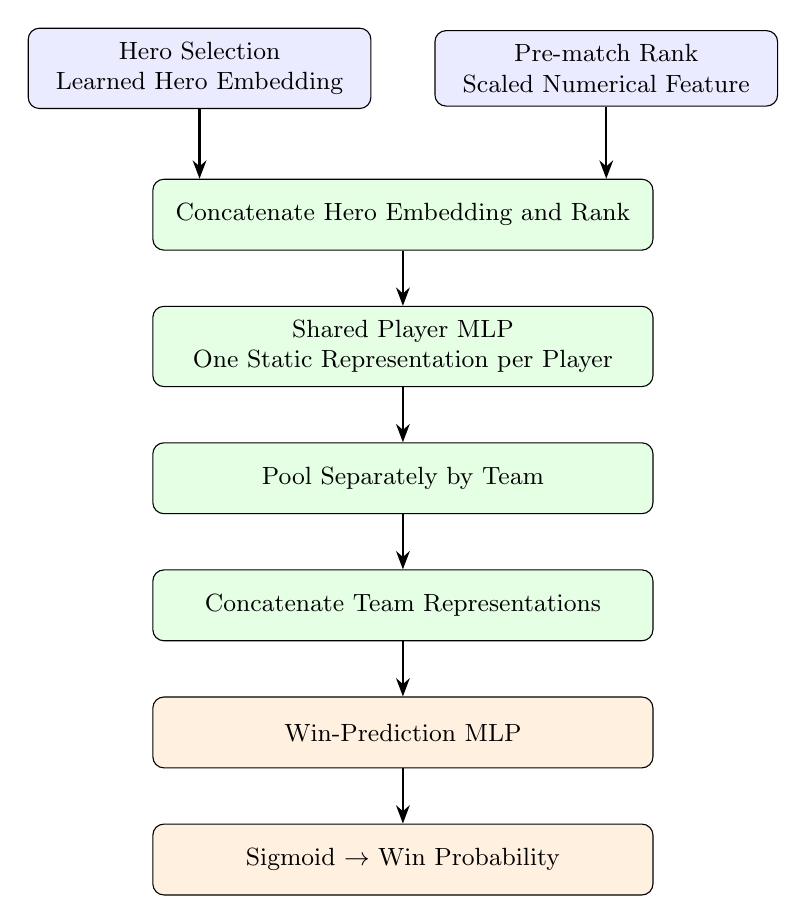
\begin{tikzpicture}[
            font=\small,
            node distance=7mm,
            box/.style={
                draw,
                rounded corners,
                align=center,
                text width=6cm,
                minimum height=9mm,
                inner sep=5pt
            },
            input/.style={box, text width=4cm, fill=blue!8},
            process/.style={box, fill=green!10},
            output/.style={box, fill=orange!12},
            arrow/.style={-{Stealth}, thick}
        ]

        \node[input] (hero) {
            Hero Selection\\
            Learned Hero Embedding
        };

        \node[input, right=8mm of hero] (rank) {
            Pre-match Rank\\
            Scaled Numerical Feature
        };

        \coordinate (middle) at
            ($(hero.south)!0.5!(rank.south)$);

        \node[process, below=9mm of middle] (concat) {
            Concatenate Hero Embedding and Rank
        };

        \node[process, below=of concat] (static) {
            Shared Player MLP\\
            One Static Representation per Player
        };

        \node[process, below=of static] (pool) {
            Pool Separately by Team
        };

        \node[process, below=of pool] (teams) {
            Concatenate Team Representations
        };

        \node[output, below=of teams] (head) {
            Win-Prediction MLP
        };

        \node[output, below=of head] (win) {
            Sigmoid $\rightarrow$ Win Probability
        };

        \draw[arrow] (hero.south) --
            (concat.north -| hero.south);
        \draw[arrow] (rank.south) --
            (concat.north -| rank.south);
        \draw[arrow] (concat) -- (static);
        \draw[arrow] (static) -- (pool);
        \draw[arrow] (pool) -- (teams);
        \draw[arrow] (teams) -- (head);
        \draw[arrow] (head) -- (win);

        \end{tikzpicture}
        \caption{
            Draft-based pre-training architecture.
            Hero embeddings and the shared player MLP are trained
            using match outcomes and transferred to Stage 2.
            Everything after the pooling is discarded.
        }
        \label{fig:pretrain1-architecture}
        \end{figure}

    \subsubsection{Loss function}
        Since this is a win-prediction task, I use binary cross-entropy between the predicted probability that team 1 wins and the observed outcome. For the sake of numerical stability, loss is computed directly from the output logit using \texttt{BCEWithLogitsLoss}.
    \subsubsection{Optimizer and learning rate}
        I use AdamW with an initial learning rate of $10^{-3}$ and initially set weight decay to zero. I may adjust the learning rate or introduce weight decay later based on validation loss.

    \subsubsection{Batch size and training duration}
        I use mini-batches of 64 matches and will train for at most 100 epochs, shuffling the training matches at each epoch. I retain the checkpoint with the lowest validation binary cross-entropy.

    \subsubsection{Regularization and stopping criteria}
        I halt if the validation loss does not improve for 10 consecutive epochs. Initially, I do not use dropouts but this may change if training loss continues to decrease while validation loss worsens. Similarly, I initially do not use weight decay, but in the event of overfitting, I will.

\subsection{Pre-Train 2 - Temporal Dynamics}
    For the second pre-training stage, I want the model to learn about game dynamics by predicting changes from the observed match history. I initialize the hero embeddings and shared player MLP from Stage 1, then train these alongside the new components.

    \subsubsection{Architecture}
% Detailed graph of training architecture for learning temporal dynamics
    \begin{figure}[H]
    \centering
    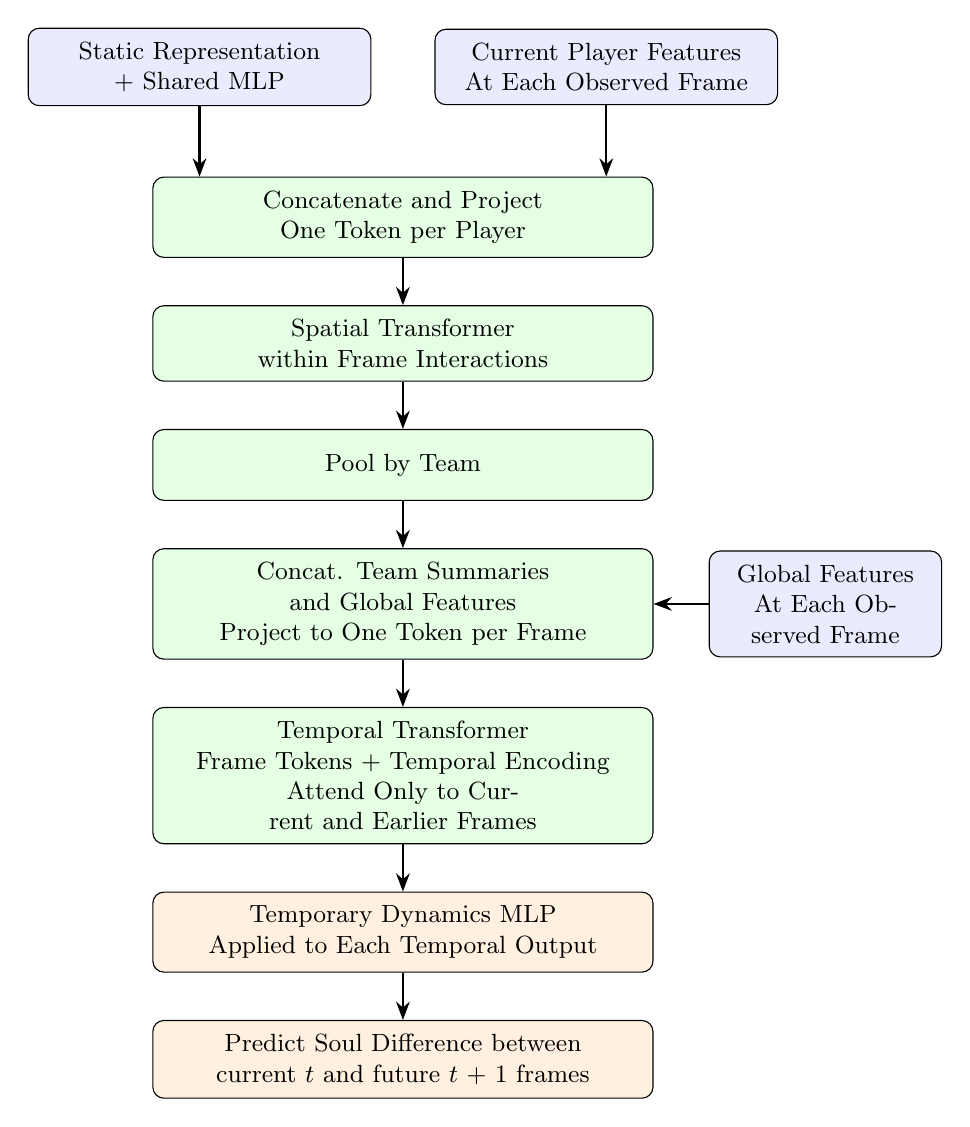
\begin{tikzpicture}[
        font=\small,
        node distance=6mm,
        box/.style={
            draw,
            rounded corners,
            align=center,
            text width=6cm,
            minimum height=9mm,
            inner sep=5pt
        },
        input/.style={box, text width=4cm, fill=blue!8},
        process/.style={box, fill=green!10},
        output/.style={box, fill=orange!12},
        arrow/.style={-{Stealth}, thick}
    ]

    \node[input] (hero) {
        Static Representation\\
        + Shared MLP
    };

    \node[input, right=8mm of hero] (state) {
        Current Player Features\\
        At Each Observed Frame
    };

    \coordinate (middle) at
        ($(hero.south)!0.5!(state.south)$);

    \node[process, below=9mm of middle] (concat) {
        Concatenate and Project\\
        One Token per Player
    };

    \node[process, below=of concat] (spatial) {
        Spatial Transformer\\
        within Frame Interactions
    };

    \node[process, below=of spatial] (pool) {
        Pool by Team
    };

    \node[process, below=of pool] (frame) {
        Concat. Team Summaries\\
        and Global Features\\
        Project to One Token per Frame
    };

    \node[input, right=7mm of frame, text width=2.6cm] (global) {
        Global Features\\
        At Each Observed Frame
    };

    \node[process, below=of frame] (temporal) {
        Temporal Transformer\\
        Frame Tokens + Temporal Encoding\\
        Attend Only to Current and Earlier Frames
    };

    \node[output, below=of temporal] (head) {
        Temporary Dynamics MLP\\
        Applied to Each Temporal Output
    };

    \node[output, below=of head] (prediction) {
        Predict Soul Difference between\\
        current $t$ and future $t+1$ frames
    };

    \draw[arrow] (hero.south) --
        (concat.north -| hero.south);
    \draw[arrow] (state.south) --
        (concat.north -| state.south);
    \draw[arrow] (concat) -- (spatial);
    \draw[arrow] (spatial) -- (pool);
    \draw[arrow] (pool) -- (frame);
    \draw[arrow] (global.west) -- (frame.east);
    \draw[arrow] (frame) -- (temporal);
    \draw[arrow] (temporal) -- (head);
    \draw[arrow] (head) -- (prediction);

    \end{tikzpicture}
    \caption{
        Dynamics pre-training architecture.
        The output at frame $t$ predicts changes over the next
        recorded interval using only frames $0{:}t$.
        All components above the temporary dynamics head
        transfer to the final win-prediction model.
    }
    \label{fig:pretrain2-architecture}
    \end{figure}
    \subsubsection{Prediction targets}
        I want to predict selected next-frame changes in continuous variables, such as position, souls, and health, together with next-frame binary states, such as whether a player is alive or an objective remains standing. I exclude fixed attributes, like hero identity, and quantities I already know, like the next timestamp. For now, I start with a simple soul-difference prediction, but I may expand this later.

    \subsubsection{Loss function}
        I use mean squared error for continuous changes, which I standardize using training-set means and standard deviations. If I add binary targets, I will use binary cross-entropy computed from logits. I average each loss over its valid targets and exclude padded frames and missing targets. If I use both target groups, I will initially give them equal weight.

    \subsubsection{Optimizer and learning rate}
        I use AdamW with an initial learning rate of $10^{-4}$ for the transferred hero embeddings and static player MLP, and $\times10^{-3}$ for newly initialized components. Initially I set weight decay to zero, but may introduce it if validation performance indicates overfitting.

    \subsubsection{Batch size and training duration}
        I start with mini-batches of 8 match sequences and will train for at most 100 epochs. I average prediction losses within each match before averaging across matches, so longer matches do not automatically receive more weight.

    \subsubsection{Regularization and stopping criteria}
        I use dropout of $0.1$ within the transformer blocks and halt if validation loss does not improve for 10 consecutive epochs. I retain the checkpoint with the lowest validation loss and clip the total gradient norm to 1 to limit unusually large updates.

    \subsubsection{Causal masking and sequence handling}
        I use causal attention so the representation at frame $t$ only uses frames $0{:}t$, then train it against targets from frame $t+1$. I mask padding in both attention and loss computation, and omit prediction at the final frame since there is no subsequent observation.

    \subsubsection{Validation and parameter transfer}
        I compare prediction errors against a simple persistence baseline, which predicts no change from the current frame, and report results separately by target group. I then transfer the player encoder, spatial transformer, frame projection, and temporal transformer to the final stage, discarding the temporary prediction heads.

\subsection{Fine-Tune - Win Prediction}
    Finally, I use the representations learned in Stage 2 to predict the winning team from a partially observed match. I replace the dynamics head with a randomly initialized win-prediction MLP, then fine-tune the entire model.

    \subsubsection{Architecture}
        I use the architecture in Figure~\ref{fig:final-architecture}, taking the temporal representation at the sampled cutoff $T$. I pass this through an MLP with dimensions $64\rightarrow32\rightarrow1$, with ReLU between layers and sigmoid to convert the final logit into a win probability.

    \subsubsection{Prediction targets and prefix sampling}
        I sample a training match uniformly, then sample a cutoff $T$ uniformly among its eligible recorded frames and give the model only frames $0{:}T$. The target is the final match outcome, encoded as 1 if team 1 wins and 0 otherwise. I exclude terminal frames and any features that explicitly reveal the outcome.

    \subsubsection{Loss function}
        As in Stage 1, I use binary cross-entropy between the predicted win probability and the observed match outcome, averaged over sampled matches. I compute this directly from logits using \texttt{BCEWithLogitsLoss}, without applying sigmoid beforehand.

    \subsubsection{Optimizer and learning rate}
        I use AdamW with an initial learning rate of $10^{-5}$ for the transferred backbone and $10^{-4}$ for the new win-prediction head. Initially, I set weight decay to zero. As before, these learning rates are starting values that I may adjust based on validation loss.

    \subsubsection{Batch size and training duration}
        I use mini-batches of 8 match prefixes and will train for at most 100 epochs, sampling a new cutoff for each training match each epoch. I pad prefixes within each batch as needed and take the temporal output at each prefix's actual cutoff, rather than at a padded position.

    \subsubsection{Regularization and stopping criteria}
        I retain transformer dropout of $0.1$ and gradient clipping at a total norm of 1. I halt if validation binary cross-entropy does not improve for 10 consecutive epochs, then restore the checkpoint with the lowest validation loss.

    \subsubsection{Causal masking and sequence handling}
        I retain causal attention and mask padded frames, so each representation only uses the available match history. I also reuse the feature scaling learned from training data; normalizing each match using its complete trajectory would give the model information about the future.

    \subsubsection{Validation}
        I keep the validation prefixes fixed so I can compare checkpoints without the added variation from new cutoffs. I report binary cross-entropy, Brier score, calibration, and AUC at fixed elapsed times, using only matches still in progress at each time.



\section{Initial Results}
    This section is a both a summary of my completed first run, and some brainstorming for next step/improvements.

\subsection{Embedding Pre-Train (Stage 1)}
\subsubsection{Summary Statistics}
    I trained the static encoder using only pre-match hero selections and ranks from the end-of-match database. 
    Table~\ref{tab:static-results} summarizes the saved run; the constant-probability reference is the BCE for
    predicting $p=0.5$ on every match.
% Pretrain 1 stat table
    \begin{table}[H]
    \centering
    \small
    \renewcommand{\arraystretch}{1.15}
    \begin{tabularx}{\textwidth}{>{\raggedright\arraybackslash}X r}
    \toprule
    \textbf{Statistic} & \textbf{Value} \\
    \midrule
    Training / validation / reserved test matches & 10,528 / 1,316 / 1,316 \\
    Selected epoch / completed epochs & 8 / 18 \\
    Validation BCE at selected checkpoint & 0.673767 \\
    Constant $p=0.5$ BCE reference & 0.693147 \\
    Training BCE: selected epoch / final epoch & 0.670678 / 0.667505 \\
    Validation BCE at final epoch & 0.677387 \\
    Missing player ranks across all splits & 91.19\% \\
    Matches with every rank missing & 11,917 / 13,160 \\
    Training rank median / minimum / maximum & 53 / 11 / 116 \\
    \bottomrule
    \end{tabularx}
    \caption{Stage 1 results and rank availability for the saved October 23 run.}
    \label{tab:static-results}
    \end{table}

\subsubsection{Issues}
    Rank information was very sparse, >90\% of observations did not have a rank. Median imputation can only do so much. 
    Also, validation loss worsened after the selected checkpoint, and training loss kept falling, so it was overfitting.

\subsubsection{Improvement}
    I need a more complex embedding structure, or a different type of training objective. Their is obvious benefit to embedding 
    clearly, hero selection is a strong predictor, but I need to find a way to get that information more reliably, and to 
    use all the information available.

    I must consider how I want to deal with the missing rank information. Either I can simply use the reduced number of runs, 
    since I already seem to have more than I need, or I can remove rank.

    I will certainly keep early stopping. But I am considering weight decay, dropouts, and learning rate decay.


\subsection{Dynamics Pre-Train (Stage 2)}
\subsubsection{Summary Statistics}
    The objective I used was to predict the next one-second change in team soul lead, $\Delta(\text{team 1 net worth}-\text{team 0 net worth})$.
    I averaged squared error within each match and then across matches, so long matches did not receive more weight. 
    Persistence predicts no change in the lead.

    \begin{table}[H]
    \centering
    \small
    \renewcommand{\arraystretch}{1.15}
    \begin{tabularx}{\textwidth}{>{\raggedright\arraybackslash}X r r}
    \toprule
    \textbf{Validation metric} & \textbf{Model} & \textbf{Persistence} \\
    \midrule
    Standardized MSE & 0.838067 & 0.953371 \\
    RMSE in souls & 403.57 & 430.44 \\
    Relative MSE reduction & 12.09\% & --- \\
    Relative RMSE reduction & 6.24\% & --- \\
    \midrule
    \multicolumn{3}{l}{\textbf{Run statistics}} \\
    Training / validation / reserved test matches & \multicolumn{2}{r}{970 / 116 / 134} \\
    Valid training / validation targets & \multicolumn{2}{r}{2,031,046 / 241,431} \\
    Selected epoch / completed epochs & \multicolumn{2}{r}{23 / 33} \\
    Training MSE: selected / final epoch & \multicolumn{2}{r}{0.839863 / 0.825801} \\
    Validation MSE at final epoch & \multicolumn{2}{r}{0.841365} \\
    Successful-run wall time & \multicolumn{2}{r}{100.6 minutes} \\
    \bottomrule
    \end{tabularx}
    \caption{Stage 2 results from the completed October 29 run. Wall time excludes
    the stopped initial attempt.}
    \label{tab:dynamics-results}
    \end{table}

\subsubsection{Issues}
    I had to make some adjustment to how the batches were loaded, as it would not fit in memory. 
    Also, there was also clear overfitting, as the validation loss was increasing while training loss was decreasing.

\subsubsection{Improvements}
    I think I'll try to reduce the learning rate for the transferred encoder. Because of overfitting, I also plan on trying 
    dropouts, weight decay, and learning rate decay. I may also try adjusting the window of prediction from 1 second to 5 seconds.


\subsection{Win-Prediction Fine-Tune}
\subsubsection{Summary Statistics}
    I conducted two runs of this fine-tune. So, I compared both runs on the same validation prefixes. Both started from the 
    same Stage 2 checkpoint, used the same seed, and retained the architecture, preprocessing, match splits, and 
    uniform per-match prefix sampling. I used the training win frequency as the constant baseline.

    \begin{table}[H]
    \centering
    \small
    \renewcommand{\arraystretch}{1.15}
    \begin{tabularx}{\textwidth}{>{\raggedright\arraybackslash}X r r r}
    \toprule
    \textbf{Validation metric} & \textbf{Prior} & \textbf{Run 1} & \textbf{Run 2} \\
    \midrule
    BCE (lower is better) & 0.692897 & 0.638630 & 0.632603 \\
    Brier score (lower is better) & 0.249875 & 0.224818 & 0.222922 \\
    AUC (higher is better) & 0.500000 & 0.680952 & 0.686012 \\
    ECE, 10 bins (lower is better) & 0.013118 & 0.083140 & 0.088072 \\
    \midrule
    \textbf{Setting / run statistic} & & \textbf{Run 1} & \textbf{Run 2} \\
    Backbone learning rate & & $10^{-5}$ & $3\times10^{-6}$ \\
    Transformer dropout & & 0.1 & 0.2 \\
    Learning-rate scheduler & & None & Plateau \\
    Rate reductions after epochs & & --- & 28, 31, 34 \\
    Selected / completed epochs & & 9 / 19 & 25 / 35 \\
    Wall time (minutes) & & 50.7 & 86.9 \\
    Training BCE at selected epoch & & 0.618717 & 0.601868 \\
    Final training BCE & & 0.561030 & 0.601634 \\
    Final validation BCE & & 0.658338 & 0.635913 \\
    \midrule
    Training / validation / reserved test & \multicolumn{3}{r}{970 / 116 / 134 matches} \\
    Run 2 relative BCE / Brier reduction & \multicolumn{3}{r}{0.94\% / 0.84\%} \\
    Paired $95\%$ interval, BCE (Run 2 $-$ Run 1) & \multicolumn{3}{r}{$[-0.03008,+0.02209]$} \\
    \bottomrule
    \end{tabularx}
    \caption{Fine-tuning comparison. The descriptive interval uses 10,000 paired
    match bootstrap resamples (seed 2026). GPU workload was not controlled
    between runs, so wall time is not a controlled throughput comparison.}
    \label{tab:finetune-results}
    \end{table}

\subsubsection{Issues}
    Both runs suffered from clear overfitting. 

\subsubsection{Improvements}
    The same as the both pretraining stages, I want to try dropouts, weight decay, and learning rate decay. 

\end{document}
